\documentclass[border=4pt]{standalone}
\usepackage{amsmath,amssymb,amsfonts}
\usepackage{xcolor,colortbl,array,booktabs,multirow}
\usepackage{tikz}
\usepackage{pgfplots}
\pgfplotsset{compat=1.16}
\usetikzlibrary{arrows, automata, backgrounds, calendar, chains, decorations,
    matrix, mindmap, patterns, petri, positioning, shadows, shapes.geometric,
    trees, shapes, decorations.pathreplacing, calc, tikzmark, arrows.meta,
    intersections, fit, graphs, quotes, angles, decorations.markings}
\newcommand{\st}{\text{ s.t. }}
\newcommand{\x}{\mathbf{x}}
\renewcommand{\b}{\mathbf{b}}
\renewcommand{\c}{\mathbf{c}}
\newcommand{\A}{\mathbf{A}}
\newcommand{\y}{\mathbf{y}}
\newcommand{\z}{\mathbf{z}}
\newcommand{\R}{\mathbb{R}}
\newcommand{\RR}{\mathbb{R}}
\newcommand{\Z}{\mathbb{Z}}
\newcommand{\ZZ}{\mathbb{Z}}
\newcommand{\npcomplete}{NP-complete}
\providecommand{\true}{\text{TRUE}}
\providecommand{\false}{\text{FALSE}}
\tikzset{vertex/.style={circle,fill=black!25,minimum size=20pt,inner sep=0pt},
    edge/.style={draw,thick,-},weight/.style={font=\small},
    selected vertex/.style={vertex, fill=red!24},
    selected edge/.style={draw,line width=2pt,-,red!50},
    ignored edge/.style={draw,line width=2pt,-,black!20}}
\newcommand{\vect}{\vec}
\providecommand{\ds}{\displaystyle}
\providecommand{\longvect}{\overrightarrow}
\usepackage[normalem]{ulem}
\definecolor{ocre}{RGB}{243,102,25}
\providecommand{\leftB}{\left[}
\providecommand{\rightB}{\right]}
\tikzset{directed/.style={postaction={decorate,decoration={markings,mark=at position .65 with {\arrow{>}}}}},
    directed1/.style={postaction={decorate,decoration={markings,mark=at position .65 with {\arrow{>}}}}}}
\begin{document}
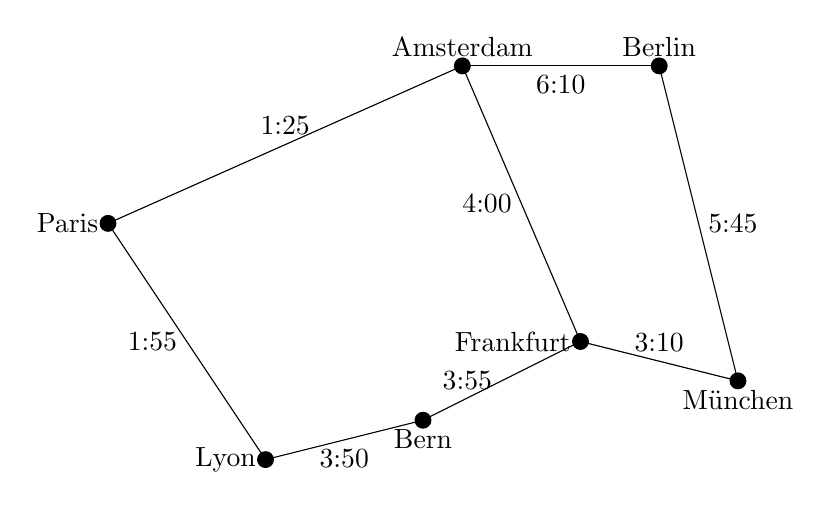
\begin{tikzpicture}
\draw[fill] (0,0) circle[radius=.1] node[left]{Paris};
\draw[fill] (2,-3) circle[radius=.1] node[left]{Lyon};
\draw[fill] (4,-2.5) circle[radius=.1] node[below]{Bern};
\draw[fill] (6,-1.5) circle[radius=.1] node[left]{Frankfurt};
\draw[fill] (8,-2) circle[radius=.1] node[below]{M\"unchen};
\draw[fill] (4.5,2) circle[radius=.1] node[above]{Amsterdam};
\draw[fill] (7,2) circle[radius=.1] node[above]{Berlin};
\draw(0,0) to node[above]{1:25} (4.5,2);
\draw(0,0) to node[left]{1:55} (2,-3);
\draw(2,-3) to node[below]{3:50} (4,-2.5);
\draw(4,-2.5) to node[left]{3:55} (6,-1.5);
\draw(6,-1.5) to node[above]{3:10} (8,-2);
\draw(6,-1.5) to node[left]{4:00} (4.5,2);
\draw(8,-2) to node[right]{5:45} (7,2);
\draw(7,2) to node[below]{6:10} (4.5,2);
\end{tikzpicture}
\end{document}
